
\section{Experimental Tools}\label{method:tools}

In order to explore the large number of possible exchange instances described in
\S \ref{method:setup}, a sophisticated problem solving framework is needed. This
section describes the design principles and implementation details of a new
software package called Cyclopts (\underline{Cycl}us \underline{Opt}imization
\underline{S}tudies). Cyclopts, written primarily in Python with a C++ layer
used to operate with Cyclus, provides a general framework for sampling a
parameter space, defining problem instances for a given point in parameter
space, and solving a problem instance under a variety of conditions.

The section begins with a short discussion on terminology in \S
\ref{method:tools:term}.  \S \ref{method:tools:struc} describes the general
Cyclopts workflow and specific features used in the DRE experimental
campaign. \S \ref{method:tools:hdf5} discusses Cyclopts persistence mechanisms,
including database design and layout. The section concludes with \S \ref{},
describing Cyclopts' high throughput computing (HTC) capability, which enables
scalable, concurrent execution.

\subsection{Terminology}\label{method:tools:term}

Cyclopts supports a two-tier definition of problem instances, borrowing terms
from biological classification. Problem \textit{families} describe a general
form of problem instance. For example, the Traveling Salesman Problem (TSP)
could be implemented as a problem family. In this analysis, the NFCTP is
considered the problem family, since any given instance of the NFCTP will have
the same general structure. Whether or not the LP or MILP formulation is used is
dependent on whether or not arcs in the Exchange Graph are labeled as exclusive
or not. If there are no exclusive arcs, the LP formulation is used; otherwise,
the MILP formulation is used.

Each problem family can have any number of \textit{species}. One can
conceptualize the relationship as a tree structure, in which families are parent
nodes and species are child nodes. A problem species defines the methodology for
generating \textit{instances} of a problem family. Using the TSP example above,
a problem species may be ``the greater Atlanta metropolitan area'', for which
the effect of regional gas prices may be studied. For the NFCTP study, front-end
and back-end exchanges form two separate species. Each species can have unique
parameters in addition to family-related parameters, is the case for the two
species studied.

\subsection{Design}\label{method:tools:struc}

The full Cyclopts stack is comprised of three phases: generation of parameter
space, generation of instances, and execution of instances. The workflow begins
with user input detailing a range of values for a set of parameters. Cyclopts
then translates the input into a parameter space by enumerating all possible
combinations of parameters. For example, if parameters $x$ and $y$ have defined
values of $[1, 2]$ and $[3, 4, 5]$, respectively, Cyclopts will generate a
parameter space comprised of six points in $(x, y)$ notation: $(1, 3)$, $(1,
4)$, $(1, 5)$, $(2, 3)$, $(2, 4)$, and $(2, 5)$. Each point is then then
provided to a problem species in order to generate one or more problem
instances. Species are expected to define defaults for all parameters as user
input may define values for only a subset of available parameters.

Given a point in parameter space, an instance can be generated. If there are any
stochastic effects during instance generation, many instances may be
generated. Again, because parameters are species dependent, the logic of
instance generation from a set of parameters is the task of a problem
species. Following instance generation, instances may be executed. Cyclopts
supports multiple solution options by design. The same instance may be solved
with both a heuristic and a full optimization solver, for example. Once an
instance of a problem is defined, it is independent of any species-level
effects. Accordingly, instance execution and related logic is the domain of
problem families. 

A summary of the high-level Cyclopts workflow and entities is presented in
Figure \ref{fig:lopts_desgin}. Note that objects generated as the workflow moves
from parameter space to instance solution form a tree structure.

\TODO{update fig}
\begin{figure}
  \begin{center}
    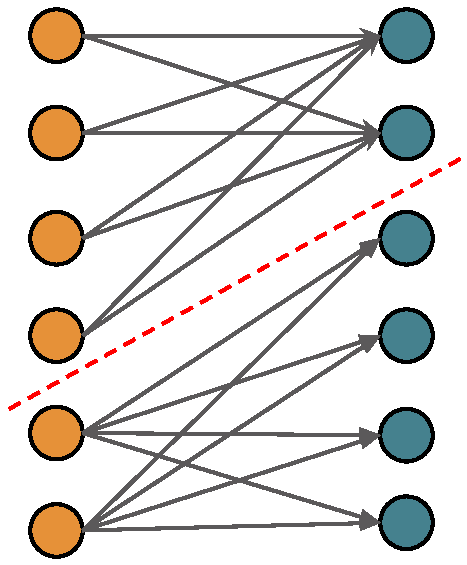
\includegraphics[width=0.55\textwidth]{exchange_part_supreq.pdf}
    \caption[]{
      \label{fig:lopts_desgin}
      Foo.}
  \end{center}
\end{figure}

\subsection{Persistence Mechanisms}\label{method:tools:hdf5}

While the root node in Figure \ref{fig:lopts_desgin} is generated from a
user-provided input file, each subsequent level in the hierarchy represents a
stateful object: a point in parameter space, a problem instance, and a
solution. Each stateful object can be written to and read from disc. Cyclopts
also incorporates a post-processing step, during which all related objects may
be analyzed and aggregate data may be collected and written to disc. While any
input/output (I/O) persistence mechanism is valid, Cyclopts is currently
implemented using Hierarchical Datat Format 5 (HDF5) \cite{hdf5} via PyTables
\cite{pytables}.

Data in HDF5 is stored hierarchicaly, similar to a filesystem. At the root node
of the filesystem-like structure, a \textit{group} is defined for problem family
and problem species data, named \code{Family} and \code{Species},
respectively. A \textit{dataset} for aggregate results named \code{Results} is
also defined. A path in HDF5 is designated in a UNIX-like manner. For example,
the path to \code{Family} would be \code{/Family}, indicating that the group is
directly under the root node, \code{/}. Further, groups are defined for each
kind of family and species. The DRE problem family records data in the group
\code{/Family/ResourceExchange}, front-end exchanges record data in the group
\code{/Species/StructuredRequest}, and back-end exchanges record data in the
group \code{/Species/StructuredSupply}. 

Each stateful object is given a Universally Unique Identifier (UUID) by which it
can be identified for future reading and analysis. The UUID is used in two
distinct capacities: as a \textit{primary key} in a dataset for future
identification or as the name of a group. Whether to aggregate data in one large
dataset or divide data into datasets for each object is a design decision
informed by practical performance. A study of the tradeoffs between each
approach is presented in \S \ref{method:tools:hdf5:study}. As a result of that
study, for objects that are both read and written, the latter approach is taken.

\subsubsection{Parameter Space}

Both front-end and back-end species record the state of every point in a given
parameter space in a data set called \code{/Species/<species type>/Points},
where \code{<species type>} is either \code{StructuredRequest} or
\code{StructuredSupply}. Each point incorporates both fundamental and instance
parameters as described in \S \ref{method:setup}.

\TODO{add table for each?}

\subsubsection{Problem Instances}

Problem instances are generated by problem species and are executed by problem
families. Accordingly, both species and families can record information about
instances. Front and back-end exchange species each record two types of
information: details about each arc in an instance and a summary of
species-specific information. The exchange family records information regarding
each of the entities that comprise an instance: nodes, groups of nodes (having
been translated from portfolios), and arcs. Further, aggregate summary
information is also recorded. 

\paragraph{Exchange Species}

Both exchange species record information about each arc in an exchange instance
detailed in Table \ref{tbl:sp_inst_arc}. A parent group for arc data is defined
under each species group. A group for each instance, whose name is the hex
string of the UUID, is defined under the associated arc group. Finally, arc
information associated with each instance is stored as a dataset in that
instance's group. For example, the arc data for a given UUID of a front-end
exchange is located as a dataset in the group
\code{/Species/StructuredRequest/Arcs/<UUID hex>}.

\begin{table}[]
\centering
\label{tbl:sp_inst_arc}
\caption{Data recorded for every arc in an instance.}
\begin{tabular}{|c|c|c|}
\hline
\textbf{Name} & \textbf{Data Type} & \textbf{Description}       \\ \hline
arcid         & 32-byte integer    & ID for an arc              \\ \hline
commod        & 32-byte integer    & ID for a commodity         \\ \hline
pref\_c       & 32-byte float      & Commodity-based preference \\ \hline
pref\_l       & 32-byte float      & Location-based preference  \\ \hline
\end{tabular}
\end{table}

Summary information related to each species is also recorded in a data set for
each species type located in the group \code{/Species/<species
  type>/Summary}. Table \ref{} describes the data recorded for front-end
exchanges, and Table \ref{} describes the data recorded for back-end exchanges.

\TODO{write both tables}

\paragraph{Exchange Family}

The exchange family records information regarding all major constructs in an
exchange: nodes, groups, and arcs. Nodes and group data are recorded in an
aggregate dataset located at \code{/Family/ResourceExchange/ExchangeNodes}. A
summary of the node datastructure is given in Tables \ref{}; the node group
data, located at \code{/Family/ResourceExchange/ExchangeGroups}, is summarized
in Table \ref{}. Arc data is collected in the group
\code{/Family/ResourceExchange/ExchangeArcs}. A dataset per instance UUID is
used because it has been found to be useful in the postprocessing phase. A
summary of the arc dataset structure is provided in Table \ref{}.

\TODO{Table for each}

\subsubsection{Solutions}

For every solution, data is added to the Cyclopts Results dataset. The structure
of the Results dataset is described in Table \ref{}. Problem solutions are
constructed from problem instances, and are thus managed by a problem
family. Aggregate solution information is provided in a family dataset
\code{/Family/ResourceExchange/ExchangeSolutionProperties}, the structure of
which is detailed in Table \ref{}. The full results of each solve, i.e., the
amount of resources flowing across each arc, are recorded in a group specific to
each solution UUID. The structure of the detailed results are provided in Table
\ref{}.

\TODO{Table for each}

\subsubsection{Post Processing}

Given a full set of parameter, instance, and solution data, postprocessing may
be applied to family and species data. The exchange family, front-end species,
and back-end species each contain a \code{PostProcess} dataset. The exchange
family dataset structure is described in Table \ref{}. Both exchange species
share the same dataset structure, outline in Table \ref{}.

\TODO{Table for each}

\subsubsection{Summary Database Layout}

The database hierarchical structure for exchange data, assuming both exchange
species are included, is shown in Figure \ref{}.

\subsubsection{Performance Studies}\label{method:tools:hdf5:study}

\textit{Chunk size} is a critical parameter of HDF5 datasets that affects I/O
performance.

In PyTables, the \textit{compresison level} is also a tuneable parameter that
affects I/O performance.

\TODO{Fix} Originally, all Cyclopts datasets used a UUID-as-primary-key
layout. However, upon the need to post process data, extremely long read times
were encountered. Originally, a chunk size of ___ was used because ___. A
compression level of four was selected per suggestions from the PyTables
documentation \cite{}.

The basic procedure for performing a post-process operation included reading all
rows associated with a UUID in an input exchange family dataset, reading all
rows associated with the same UUID in an output exchange species dataset,
selecting a value from each row, and performing a dot product of the resulting
vectors. The pseudocode for the operation is shown in Listing \ref{}.
\TODO{Make listing}

In order to investigate possible chunk size and compression optimizations, a
small ($\sim$ MBs) dataset and a large ($\sim$ GBs) dataset were created. The
postprocessing step was then run on 25 instances in each dataset. The operation
was timed using the UNIX \code{time} command.

\TODO{Discuss results}

\TODO{Discuss node v grp}

\subsection{Implementation}

Cyclopts defines abstract application programming interfaces (APIs) for both
families and species in the \code{ProblemFamily} and \code{ProblemSpecies}
classes, respectively. While many parts of an API are related to the workflow
discussed in \S \ref{method:tools:struc:des}, others are related to the
persistence mechanisms discussed in \S \ref{method:tools:hdf5}.

\subsubsection{Problem Family}

Problem families are responsible for reading instances from a database, executing instances given a solver configuration, and writing solution 

\subsubsection{Problem Species}
 
\subsubsection{Exchange Family and Species}

\subsection{High Throughput Computing}\label{method:tools:htc}

Things \cite{bui_work_2011}.

\subsection{Command Line Interface}
